\documentclass[tikz]{standalone}
\usepackage{amsfonts}
\definecolor{morange}{RGB}{255,127,14}
\definecolor{mblue}{RGB}{31,119,180}
\definecolor{mred}{RGB}{214,39,40}
\definecolor{mpurple}{RGB}{148,103,189}
\definecolor{mgreen}{RGB}{44,160,44}

\begin{document}
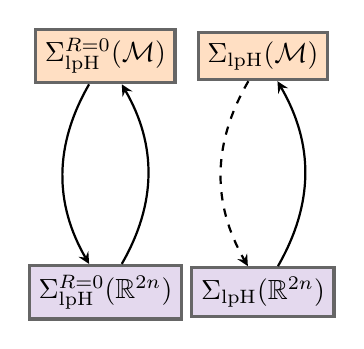
\begin{tikzpicture}[
    node1/.style={rectangle, draw=black!60, fill=mpurple!25, very thick, minimum size=5mm},
    node2/.style={rectangle, draw=black!60, fill=morange!25, very thick, minimum size=5mm},
    arrow_working/.style={-stealth, thick, rounded corners},
    arrow_open_question/.style={arrow_working, dashed},
    ]

\node[node1] (rlph1) {$\Sigma_\mathrm{lpH}^{R=0}(\mathbb{R}^{2n})$};
\node[node1, left of=rlph1, xshift = 3cm] (rlph2) {$\Sigma_\mathrm{lpH}(\mathbb{R}^{2n})$};
\node[node2, above of=rlph1, yshift = 2cm] (flph1) {$\Sigma_\mathrm{lpH}^{R=0}(\mathcal{M})$};
\node[node2, above of=rlph2, yshift = 2cm] (flph2) {$\Sigma_\mathrm{lpH}(\mathcal{M})$};

\draw[arrow_working] (rlph1) to [bend right = 30] (flph1);
\draw[arrow_working] (flph1) to [bend right = 30] (rlph1);
\draw[arrow_working] (rlph2) to [bend right = 30] (flph2);l
\draw[arrow_open_question] (flph2) to [bend right = 30] (rlph2);

\end{tikzpicture}
\end{document}